

% Gradient Info
  
\tikzset{_4uge22sc3/.code = {\pgfsetadditionalshadetransform{ \pgftransformshift{\pgfpoint{81.84 bp } { -103.62 bp }  }  \pgftransformscale{1.32 }  }}}
\pgfdeclareradialshading{_bq41dibr6}{\pgfpoint{-72bp}{88bp}}{rgb(0bp)=(1,1,1);
rgb(0.052081516810825894bp)=(1,1,1);
rgb(25bp)=(0.74,0.74,0.74);
rgb(400bp)=(0.74,0.74,0.74)}
\tikzset{every picture/.style={line width=0.75pt}} %set default line width to 0.75pt        

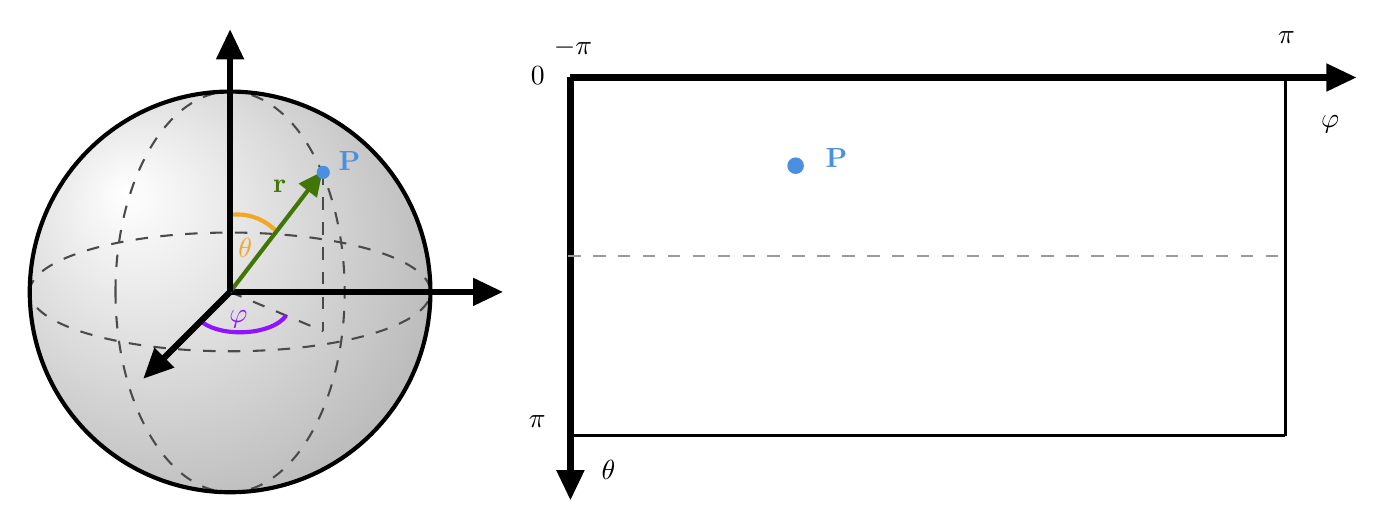
\begin{tikzpicture}[x=0.75pt,y=0.75pt,yscale=-1,xscale=1]
%uncomment if require: \path (0,313); %set diagram left start at 0, and has height of 313

%Shape: Circle [id:dp5460928729364494] 
\draw  [draw opacity=0][shading=_bq41dibr6,_4uge22sc3][line width=1.5]  (6,158.81) .. controls (6,105.5) and (49.22,62.28) .. (102.52,62.28) .. controls (155.83,62.28) and (199.05,105.5) .. (199.05,158.81) .. controls (199.05,212.12) and (155.83,255.33) .. (102.52,255.33) .. controls (49.22,255.33) and (6,212.12) .. (6,158.81) -- cycle ;
%Straight Lines [id:da5671603358142259] 
\draw [color={rgb, 255:red, 74; green, 74; blue, 74 }  ,draw opacity=1 ] [dash pattern={on 4.5pt off 4.5pt}]  (102.52,158.81) -- (147.41,177.74) ;
%Shape: Ellipse [id:dp6506733150555541] 
\draw  [color={rgb, 255:red, 74; green, 74; blue, 74 }  ,draw opacity=1 ][dash pattern={on 4.5pt off 4.5pt}] (47.31,158.81) .. controls (47.31,105.5) and (72.03,62.28) .. (102.52,62.28) .. controls (133.02,62.28) and (157.74,105.5) .. (157.74,158.81) .. controls (157.74,212.12) and (133.02,255.33) .. (102.52,255.33) .. controls (72.03,255.33) and (47.31,212.12) .. (47.31,158.81) -- cycle ;
%Shape: Ellipse [id:dp26678317589757317] 
\draw  [color={rgb, 255:red, 74; green, 74; blue, 74 }  ,draw opacity=1 ][dash pattern={on 4.5pt off 4.5pt}][line width=0.75]  (6,158.81) .. controls (6,143.01) and (49.22,130.21) .. (102.52,130.21) .. controls (155.83,130.21) and (199.05,143.01) .. (199.05,158.81) .. controls (199.05,174.6) and (155.83,187.41) .. (102.52,187.41) .. controls (49.22,187.41) and (6,174.6) .. (6,158.81) -- cycle ;
%Straight Lines [id:da95744507209868] 
\draw [line width=2.25]    (102.52,158.81) -- (228.85,158.81) ;
\draw [shift={(233.85,158.81)}, rotate = 180] [fill={rgb, 255:red, 0; green, 0; blue, 0 }  ][line width=0.08]  [draw opacity=0] (14.29,-6.86) -- (0,0) -- (14.29,6.86) -- cycle    ;
%Straight Lines [id:da9220607301798066] 
\draw [color={rgb, 255:red, 74; green, 74; blue, 74 }  ,draw opacity=1 ] [dash pattern={on 4.5pt off 4.5pt}]  (147.41,101.21) -- (147.41,177.74) ;
%Shape: Arc [id:dp11613747224217108] 
\draw  [draw opacity=0][line width=1.5]  (129.44,170.31) .. controls (126.23,174.93) and (117.42,178.27) .. (107.29,178.27) .. controls (98.97,178.27) and (91.86,176.02) .. (88.16,172.65) -- (108.09,166.89) -- cycle ; \draw  [color={rgb, 255:red, 144; green, 19; blue, 254 }  ,draw opacity=1 ][line width=1.5]  (129.44,170.31) .. controls (126.23,174.93) and (117.42,178.27) .. (107.29,178.27) .. controls (98.97,178.27) and (91.86,176.02) .. (88.16,172.65) ;
%Shape: Arc [id:dp1998195952216596] 
\draw  [draw opacity=0][line width=1.5]  (101.94,121.87) .. controls (103.31,121.62) and (104.73,121.49) .. (106.19,121.49) .. controls (113.22,121.49) and (119.81,124.53) .. (124.6,129.37) -- (108.34,145.32) -- cycle ; \draw  [color={rgb, 255:red, 245; green, 166; blue, 35 }  ,draw opacity=1 ][line width=1.5]  (101.94,121.87) .. controls (103.31,121.62) and (104.73,121.49) .. (106.19,121.49) .. controls (113.22,121.49) and (119.81,124.53) .. (124.6,129.37) ;
%Straight Lines [id:da3798410950733011] 
\draw [color={rgb, 255:red, 65; green, 117; blue, 5 }  ,draw opacity=1 ][line width=1.5]    (102.52,158.81) -- (144.58,103.99) ;
\draw [shift={(147.01,100.81)}, rotate = 487.49] [fill={rgb, 255:red, 65; green, 117; blue, 5 }  ,fill opacity=1 ][line width=0.08]  [draw opacity=0] (11.61,-5.58) -- (0,0) -- (11.61,5.58) -- cycle    ;
%Shape: Ellipse [id:dp5016585286703897] 
\draw  [draw opacity=0][fill={rgb, 255:red, 74; green, 144; blue, 226 }  ,fill opacity=1 ] (144.23,101.21) .. controls (144.23,99.46) and (145.66,98.03) .. (147.41,98.03) .. controls (149.17,98.03) and (150.59,99.46) .. (150.59,101.21) .. controls (150.59,102.97) and (149.17,104.39) .. (147.41,104.39) .. controls (145.66,104.39) and (144.23,102.97) .. (144.23,101.21) -- cycle ;
%Straight Lines [id:da5083339397538952] 
\draw [line width=2.25]    (102.52,158.81) -- (64.35,196.98) ;
\draw [shift={(60.82,200.52)}, rotate = 315] [fill={rgb, 255:red, 0; green, 0; blue, 0 }  ][line width=0.08]  [draw opacity=0] (14.29,-6.86) -- (0,0) -- (14.29,6.86) -- cycle    ;
%Straight Lines [id:da9550893076013829] 
\draw [line width=2.25]    (102.52,158.81) -- (102.52,37.47) ;
\draw [shift={(102.52,32.47)}, rotate = 450] [fill={rgb, 255:red, 0; green, 0; blue, 0 }  ][line width=0.08]  [draw opacity=0] (14.29,-6.86) -- (0,0) -- (14.29,6.86) -- cycle    ;
%Shape: Circle [id:dp9507399492507013] 
\draw  [line width=1.5]  (6,158.81) .. controls (6,105.5) and (49.22,62.28) .. (102.52,62.28) .. controls (155.83,62.28) and (199.05,105.5) .. (199.05,158.81) .. controls (199.05,212.12) and (155.83,255.33) .. (102.52,255.33) .. controls (49.22,255.33) and (6,212.12) .. (6,158.81) -- cycle ;
%Straight Lines [id:da03703665360269759] 
\draw [line width=2.25]    (266.5,55.5) -- (640,55.5) ;
\draw [shift={(645,55.5)}, rotate = 180] [fill={rgb, 255:red, 0; green, 0; blue, 0 }  ][line width=0.08]  [draw opacity=0] (14.29,-6.86) -- (0,0) -- (14.29,6.86) -- cycle    ;
%Straight Lines [id:da4086515257550415] 
\draw [line width=2.25]    (266.5,55.5) -- (266.5,254) ;
\draw [shift={(266.5,259)}, rotate = 270] [fill={rgb, 255:red, 0; green, 0; blue, 0 }  ][line width=0.08]  [draw opacity=0] (14.29,-6.86) -- (0,0) -- (14.29,6.86) -- cycle    ;
%Straight Lines [id:da3388765743708252] 
\draw    (265.42,228) -- (611,228) ;
%Straight Lines [id:da4093781654104244] 
\draw    (611,228) -- (611,55) ;
%Straight Lines [id:da3339822614948319] 
\draw [color={rgb, 255:red, 155; green, 155; blue, 155 }  ,draw opacity=1 ] [dash pattern={on 4.5pt off 4.5pt}]  (265.42,141.5) -- (611,141.5) ;
%Shape: Circle [id:dp8218466607420762] 
\draw  [draw opacity=0][fill={rgb, 255:red, 74; green, 144; blue, 226 }  ,fill opacity=1 ] (371,98) .. controls (371,95.79) and (372.79,94) .. (375,94) .. controls (377.21,94) and (379,95.79) .. (379,98) .. controls (379,100.21) and (377.21,102) .. (375,102) .. controls (372.79,102) and (371,100.21) .. (371,98) -- cycle ;

% Text Node
\draw (121.75,103.33) node [anchor=north west][inner sep=0.75pt]  [color={rgb, 255:red, 65; green, 117; blue, 5 }  ,opacity=1 ] [align=left] {$\displaystyle \mathbf{r}$};
% Text Node
\draw (112.43,177.54) node [anchor=south east] [inner sep=0.75pt]  [color={rgb, 255:red, 144; green, 19; blue, 254 }  ,opacity=1 ] [align=left] {$\displaystyle \mathbf{\varphi }$};
% Text Node
\draw (109.84,137.5) node  [color={rgb, 255:red, 245; green, 166; blue, 35 }  ,opacity=1 ] [align=left] {$\displaystyle \mathbf{\theta }$};
% Text Node
\draw (153.33,89.83) node [anchor=north west][inner sep=0.75pt]  [color={rgb, 255:red, 74; green, 144; blue, 226 }  ,opacity=1 ] [align=left] {$\displaystyle \mathbf{P}$};
% Text Node
\draw (257,35) node [anchor=north west][inner sep=0.75pt]   [align=left] {$\displaystyle -\pi $};
% Text Node
\draw (606,32) node [anchor=north west][inner sep=0.75pt]   [align=left] {$\displaystyle \pi $};
% Text Node
\draw (245,217) node [anchor=north west][inner sep=0.75pt]   [align=left] {$\displaystyle \pi $};
% Text Node
\draw (246,49) node [anchor=north west][inner sep=0.75pt]   [align=left] {$\displaystyle 0$};
% Text Node
\draw (388,88) node [anchor=north west][inner sep=0.75pt]  [color={rgb, 255:red, 74; green, 144; blue, 226 }  ,opacity=1 ] [align=left] {$\displaystyle \mathbf{P}$};
% Text Node
\draw (638.43,83.54) node [anchor=south east] [inner sep=0.75pt]  [color={rgb, 255:red, 0; green, 0; blue, 0 }  ,opacity=1 ] [align=left] {$\displaystyle \mathbf{\varphi }$};
% Text Node
\draw (284.84,244.5) node  [color={rgb, 255:red, 0; green, 0; blue, 0 }  ,opacity=1 ] [align=left] {$\displaystyle \mathbf{\theta }$};


\end{tikzpicture}

